
% Language setting
% Replace `english' with e.g. `spanish' to change the document language
\usepackage[english]{babel}

% Set page size and margins
% Replace `letterpaper' with `a4paper' for UK/EU standard size
\usepackage[letterpaper,top=2cm,bottom=2cm,left=3cm,right=3cm,marginparwidth=1.75cm]{geometry}

% Useful packages
\usepackage{amsmath}
\usepackage{graphicx}
\usepackage[colorlinks=true, allcolors=blue]{hyperref}

\title{CS 6000 Git Assignment}
\author{Pi Chandramouli}


\maketitle


\section{Introduction}

Hello, my name is Pi Chandramouli. I am currently doing my Masters of Engineering in Computer Security. I have been doing research for the past 2 years and I have also published a couple of papers. In this course, I would like to learn to become a better writer. So far, all my papers are with me as a secondary author, and I have lots of projects in mind that I would like to publish as the primary author. I hope to write my own research paper, and keep getting feedback for it over the course of the semester to keep improving and working on improving the data to make it publishing ready.

\begin{figure}[!htb]
\centering
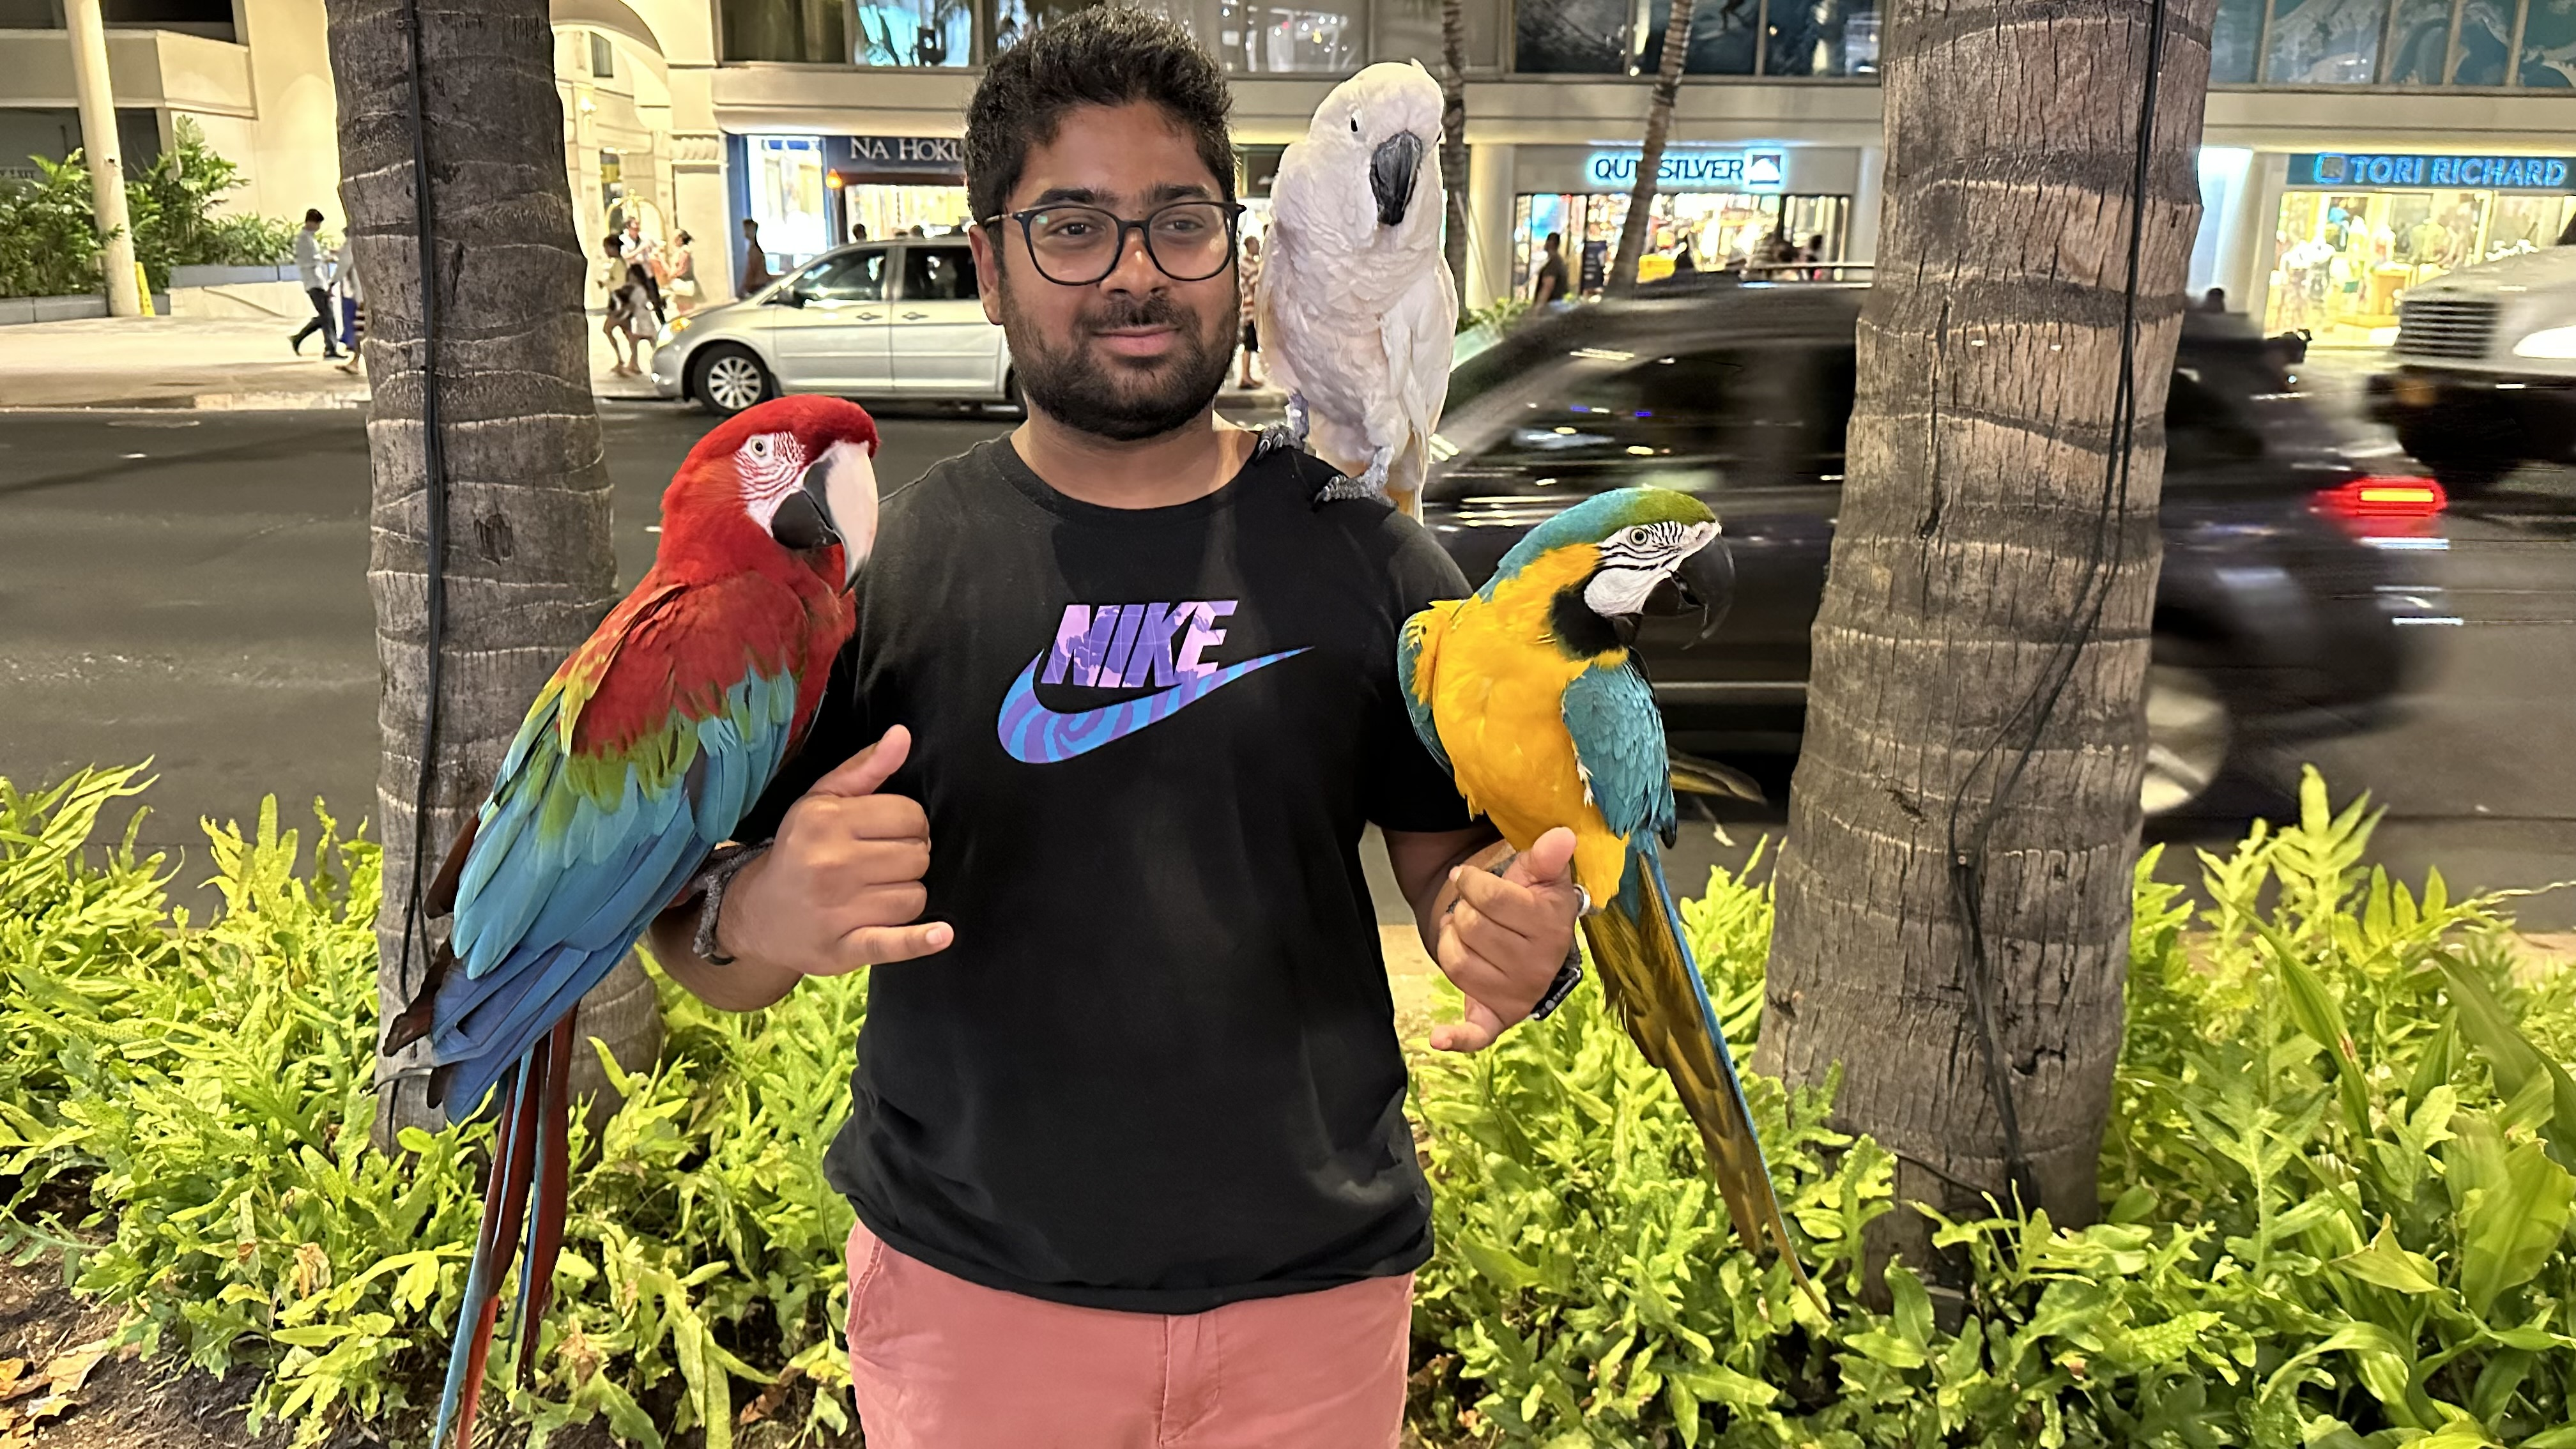
\includegraphics[width=0.5\columnwidth]{pi-F23.jpeg}
\caption{\label{fig:me} Picture of me.}
\end{figure}

I have a lot of hobbies including hiking, skiing, and running my cryptocurrency mining company. I love reading research papers/ white papers of new cryptocurrency coins to see which new problems the coin is looking to solve, and then figure out a way to mine the coin before it is known to most people. 

I look forward to learning more in this class, and learning more tips to writing better papers.

\subsection{GitHub code for Liboqs for post-quantum libraries}
Liboqs is an open source C library \nolinkurl{https://github.com/open-quantum-safe/liboqs} by Open Quantum Safe (OQS). This library can also be installed along with OpenSSL to enable post-quantum certificate generation for TCP/TLS1.3 testing, and to be used in real world certificate authorities. Once the build file is created with the compile process, engineers can use the test command to test sign and verify time of post-quantum algorithms to gather a better understanding on which algorithm to use in different situation.

\subsection{Questions}

\subsubsection{Question1}

\subsubsection{Question2}
